\documentclass[../main.tex]{subfiles}
\begin{document}
This chapter reports the development process for the software Dashboard, starting from explaining the requirements for the software Dashboard and how this tool helps developer in the process of generating software for motor \gls{ECUM}s. The chapter follows the path towards the construction of the Dashboard based on the data flow inside the pipeline that brings always updating data to the Dashboard itself. The chapter is organized based on the three main points, starting from the data source to the database organization all the way to introducing the structure of the Dashboard.
\section{Dashboard objective definition}
As already introduced in the Thesis abstract the development of \gls{ECU} software is a complex process. As each complex process composed by multiple step there is always the requirement of tracking results, quality and completeness of each step. In order to do that a high load of data is generated during each step.
In the development of \gls{ECU} software most of the steps to create output artifacts are divided over multiple departments and then additionally divided between the single member of each department. Each of the person responsible for a single task keep track of the data of that single task. Most of the time only single person know where the data for the single task lays and also how to read those data. This can be problematic especially when people that are responsible from different task require information about another one, out of their competence. They always need to refer to the person in charge. A centralized view on the process is missing, as well as a centralize storing repository for the data. \\
In order to solve the previous problem, the idea is to create a database to store data in a readable form and then to create graphical visualization, namely Dashboard of the data.\\
Via a Dashboard with updated data different developers in different teams can simultaneously surf through data and get real time information on the status of the process, thus increasing the feedback on every task and therefor the output result.
\subsection{Data pipeline concept}
The concept of having data flowing from the source that generates the data all the way to the Dashboard can be summarized under the name pipeline. This gives an idea on the basic concept that the data flow need to have. Data need to be always updated, the flow need to be controlled by some mechanism that take the updating data and push it to the different steps of the pipe up to the end step, the Dashboard itself. Three main steps can be identified in the pipeline, as also reported in Figure \ref{fig:pipelinestructure} and in Figure \ref{fig:pipeline1}:

\tikzstyle{block} = [draw, rectangle, text width=3.5cm, text centered, minimum height=1.2cm, node distance=6cm]
\begin{figure}[h]
  \centering
\begin{tikzpicture}[scale=0.85,transform shape]
    \node [block, name=text1] {Data Source};
    \node [block, right of=text1] (text2) {Data Storage};
    \node [block, right of=text2] (text3) {Data Visualization};

    \draw [->] (text1) -- (text2);
    \draw [->] (text2) -- node {} (text3);

\end{tikzpicture}
  \caption{General pipeline structure}
  \label{fig:pipelinestructure}
\end{figure}

\begin{itemize}
    \item Data source, in this case the data source is the EA-build software. As reported in Section \ref{sec:EA-buildsection} the software is responsible for the compilation, quality checking and integration of the code and therefor for the generation of the data. 
    \item Data storage, the data generated in the first step is stored in a relational database, namely EA-Dashboard. This database is the middleman between the data source and the Dashboard. The database receives information from the data source, stores the information under in tables and deliver data to the Dashboard.
    \item Data visualization, the data stored in the database gets queried and reorganized. An interactive visualization is created in a interactive manner, creating the Dashboard available for the developers team.
\end{itemize}
\begin{figure}[h]
    \centering
    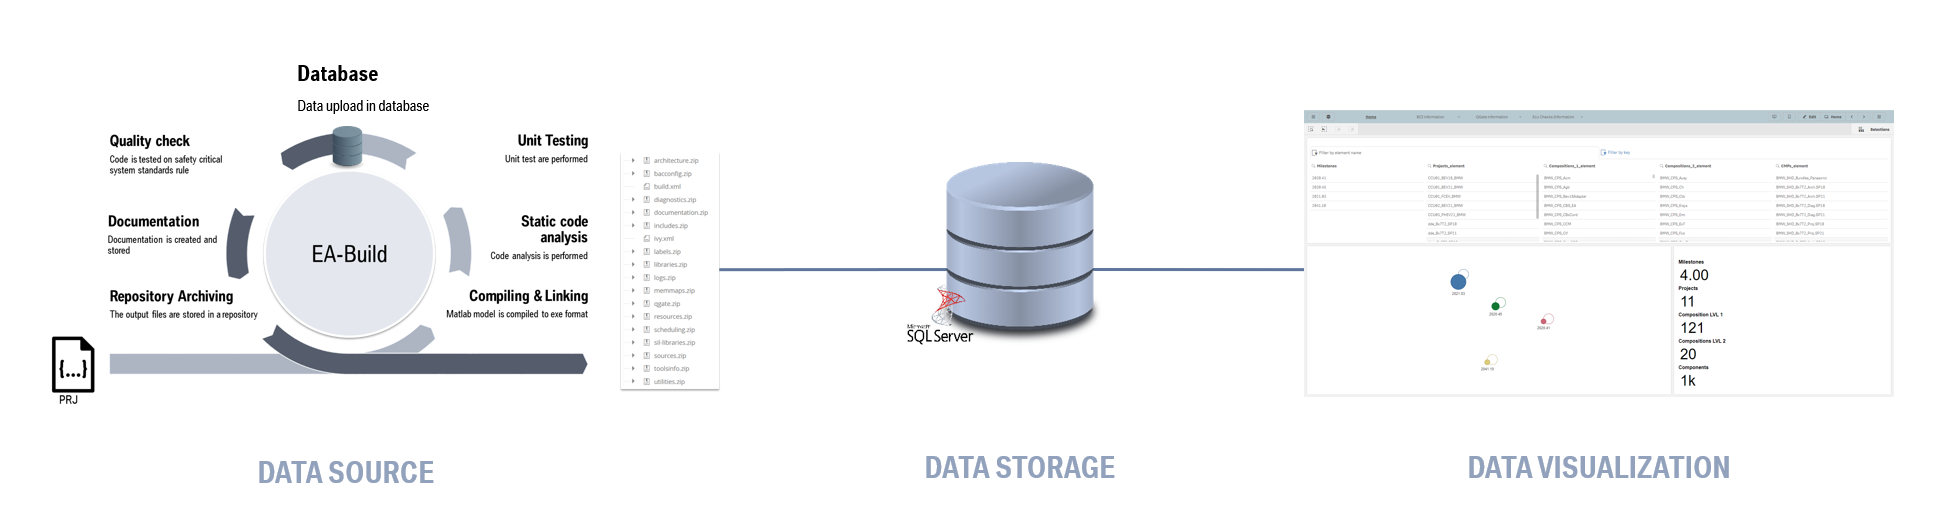
\includegraphics[width=\linewidth]{images_folder/pipeline_1.png}
    \caption{Pipeline structure}
    \label{fig:pipeline1}
\end{figure}
\section{Data Source}\label{sec:datasource}
The data source step is the one in charge of generating data. The software generating data is already been described in \ref{sec:EA-buildsection}. 
\subsection{Software structure for ECU}
In order to better understand the where the high load of data comes form and how all the data is structured, the overview on the hierarchical model of the software for \gls{ECUM} is given. The hierarchical structure is also being used as the backbone for the database organization, to connect data together.
As already described in Section \ref{sec:EA-buildsection} Software for \gls{ECU} is not developed as a single package. The hierarchical structure is composed by four different layer, with some exception to add to it. The four level present are the following and are also reported in \ref{fig:bcidashboard}, where the hierarchical structure (right side) can be seen connected to a graphical selector for the same hierarchy present in the dashboard (left side).
\begin{figure}[h]
    \centering
    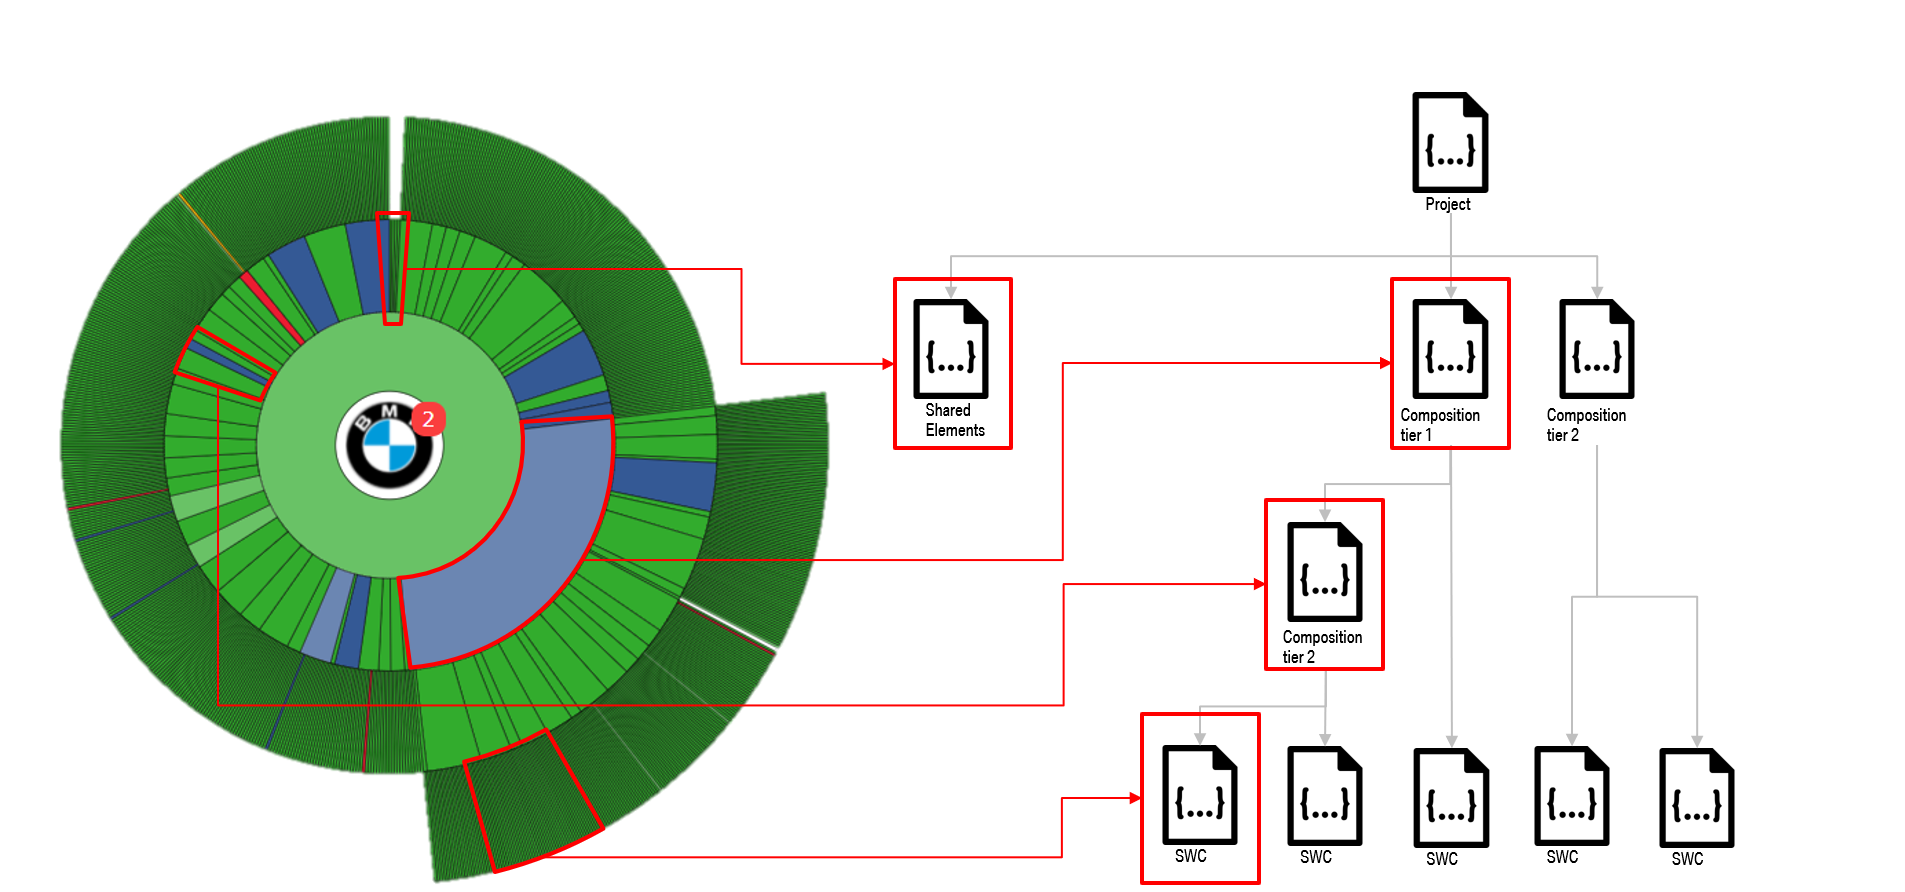
\includegraphics[width=\linewidth]{images_folder/bci_structure.png}
    \caption{Hierarchical structure}
    \label{fig:bcidashboard}
\end{figure}
The hierarchy reported in Figure \ref{fig:bcidashboard} is composed by:
\begin{itemize}
    \item SWC, software components, this is the basic block, and describes a function for a single part of the motor. It is components by multiple files, but the most important one is the runnable, which contain the logic of the function. An example of SWC can be the logic behind the control of windshield wipers or, in relation to the engine the control of the single injector. A thing to keep in mind is that the same SWC can be integrated under different version in different projects. For example the Diesel engine and the Petrol engine may share the same flow control valve, therefor the SWC responsible for the control is the same and integrated in both the motor with different specification, defined in the so-called shared element, that are instead project related
    \item Compositions tier 2, a composition is a collection of SWC. A tier 2 composition is a composition that does not have any other composition under it. An example for a composition can be the sum of all the SWCs that control the injection. In terms of software a composition is said to be successfully build when, after having compiled every SWC under it, the integration of all this components is also successfully build, meaning that the code from the different SWCs interact correctly together.
    \item Compositions tier 1, the concept is the same as the composition tier 2, but in this case a composition of tier 1 can have also other compositions under it. This happen in just seldom cases, with complex part of the control.
    \item Shared elements, shared elements are one of the exceptions. They have the same structure as a SWC, so they contain runnable but are project specific. They are software components that need to be shared by all the elements and allow for functionality specific of the project. A easy way to thing of a shared element is like a method that every SWC can call and depends on the project the SWC is integrated in.
    \item Project, refer to the collection of all compositions, components and shared element and represent a package that can be flashed on the \gls{ECUM}. If a project compile, then all the element that lay under it compile and integrate as well, and therefor the project is ready to be deployed. 
\end{itemize}
Each project is the output of the developer team, which working in Scrum update every two weeks a certain number of SWCs, thus updating every project that has that particular SWCs in it. As it is easy to thing, every time a SWCs gets an update this trigger a cascade of software build that goes all the way to the project level, and therefor creating a continuously updating load of data. Project are defined by a name and by the specif milestone that they are related to, as reported in Figure \ref{fig:SWsTR}.
\begin{figure}
    \centering
    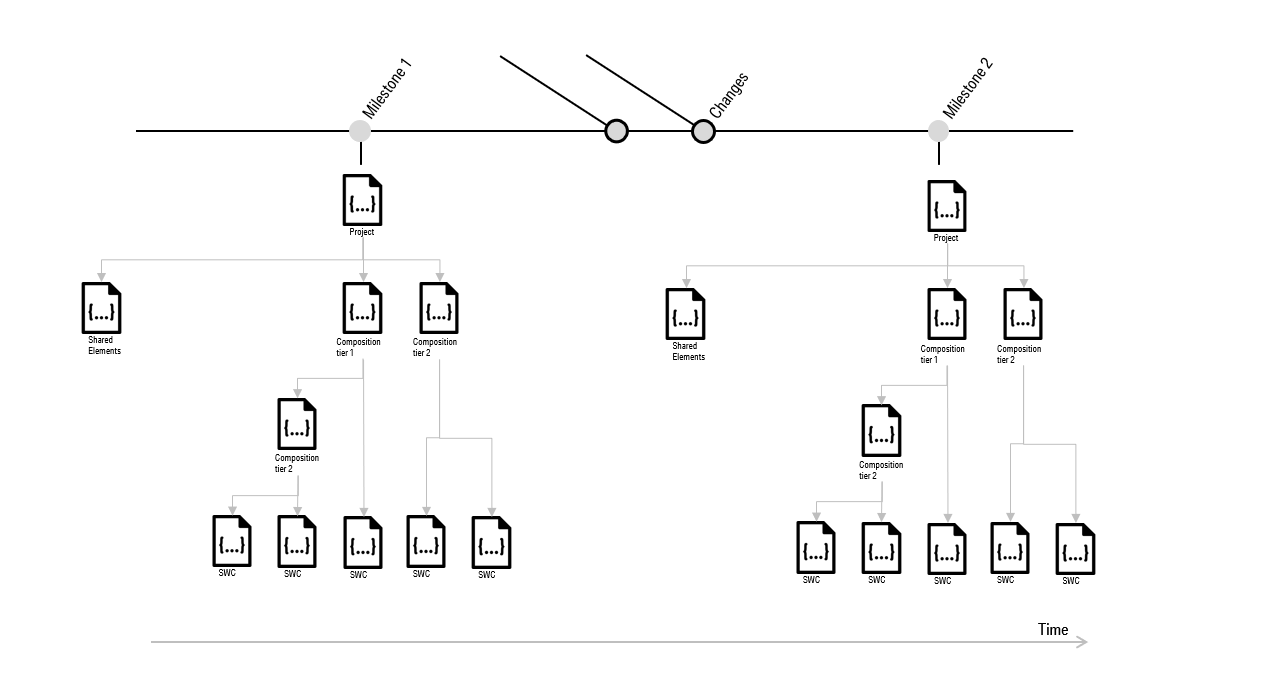
\includegraphics[width=\linewidth]{images_folder/softwarestrucutre.png}
    \caption{Software structure}
    \label{fig:SWsTR}
\end{figure}
The structure is used as the backbone for the data organization, since all the data is related to one of the hierarchy components.
\subsection{Automatic data generation}
The data generation process is the previously described part. The data is already there in the EA-build and gets generated every build run. Most of the time, as already mentioned the data gets stored under different formats, each of which is developer friendly, meaning that each developer know his own part of the data, and autonomously decides under which format to store the data. 
In order to centralize the data the integration of the capabilities to store this data in a database have been introduced in the build. The process for integrating the automatic data generation to the database have been the following:
\begin{itemize}
    \item Creation of a database integration package, creation of a package to integrate database connectivity in the already present EA-build Python software.
    \item Standardization in the mechanism for database update, define a time efficient way to have always updating data flowing to the database. 
    \item Integration of data, workflow for the integration of new data inside the database.
\end{itemize}
\subsubsection{Creation of a database integration package}
The database package is the Python package which inside the build process is responsible for storing the definition of tables, following SQLAlchemy (Section \ref{sec:SQLACHMEYMSEC}).
The structure that allow to have a data going through the software to the database is the following:
\begin{itemize}
    \item Each table has a own class, based on \gls{ORM} layer a connection is created between the database table and the python native class. 
    \item A class responsible for storing connection parameter is present, in this class are stored information such as the ip address of the database, the port as well as the user for the server and database access. Different table uses different users related to different database schemas. 
    \item Each connection has a own semaphore on the flow stream, that is the so-called \texttt{Session}, that creates a holding zone for the created objects. An example is reported in \ref{lst:code_direct}.
        \lstset{language=Python}
        \lstset{frame=lines}
        \lstset{caption={Example of Session usage}}
        \lstset{label={lst:code_direct}}
        \lstset{basicstyle=\footnotesize}
        \begin{lstlisting}
            from sqlalchemy.orm import Session
            
            # create session and add objects
            with Session(someclass.engine) as session:
                session.add(some_object)
                session.add(some_other_object)
                session.commit()
        \end{lstlisting}
\end{itemize}
\subsubsection{Standardization of the database update mechanism}
Most of the data in the Dashboard has an update periodicity of twenty minutes. This is related to the fact that update or changes in the software that trigger a rebuild are mainly checked every twenty minutes. This mean that the data to store exponentially increases. Therefor having a fast updating mechanism in the classic form, that checks what data is present and update only the data that changes is not feasible, or mostly not needed since in the Dashboard the main focus is on a feedback directed to the current status of the software.\\
Based on that the update mechanism has been translated to a so-called renew mechanism. The term renew mean that the tables gets fully overwritten every times new data comes in. Thus deleting old data and updating as a bulk the new one.\\
It need to be underlined that the storage requirement highlighted at the beginning are still valid. Thus to full-fill this requirement, while keeping the data volume on the "production database" (real time data one) as low as possible a second database instance is created, namely "EA-Dashboard-storage". This database is updated from the "production" database once day (at night, when the load on servers is lower), creating copies of all the tables and adding time stamping to the data, in order to keep track of the software status not only in a real time  but also by having historic data on software versions. This database is not still connected to any Dashboard or visualization. Therefor is as of today not possible to check the time evolution of the data. 
\begin{figure}
    \centering
    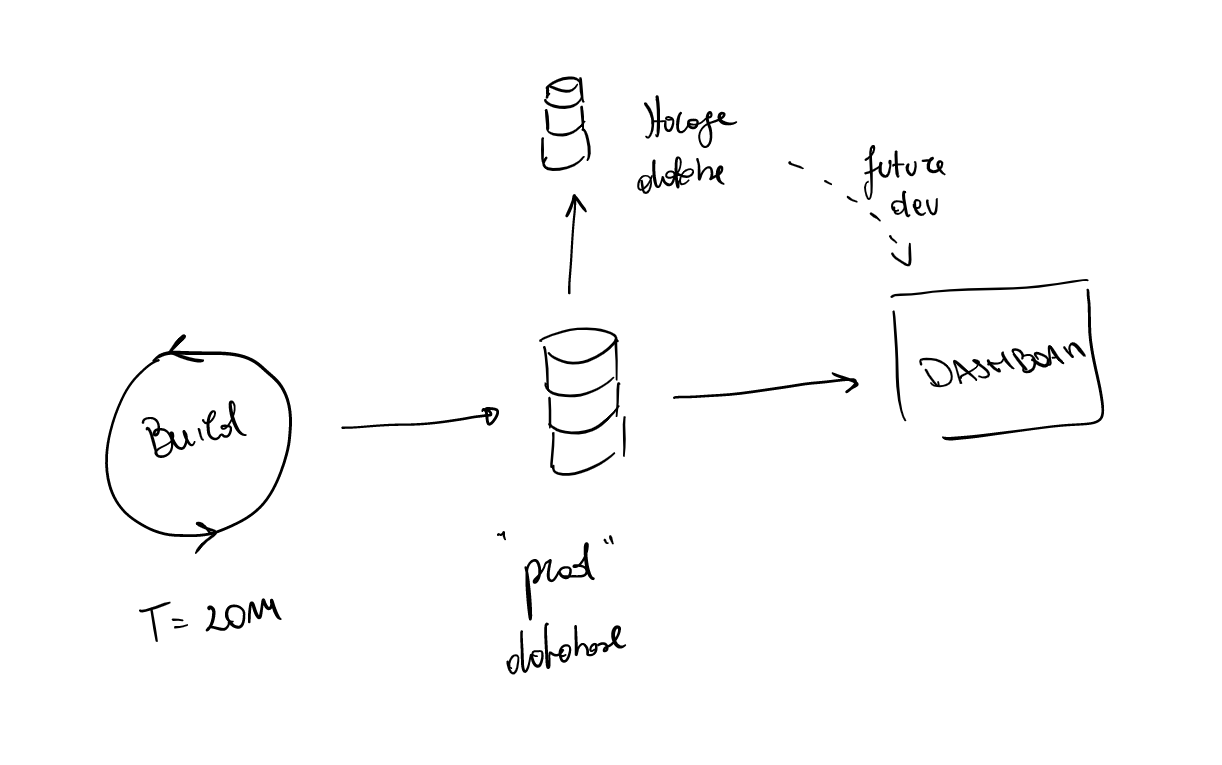
\includegraphics[width=\linewidth]{images_folder/dual_db.png}
    \caption{Double database structure}
    \label{fig:dds}
\end{figure}
\subsubsection{Integration of data}
In order to have new data inside the database and so flowing throughout the pipeline to be analyzed and displayed in the Dashboard additional steps are required. Once the developer, together with the person in charge of the Dashboard development decide that new data need be inserted in the process they follow the this procedure:
\begin{itemize}
    \item The developer highlight the data to the person in charge of integration, the main point that need to discussed is how the data gets connected to what already present in the pipeline (choice of primary key).
    \item The integration person creates a class for the new data that connect to a table object in the database. The class is then integrated in the code part that generate the data, so that once the data is generated it is also send to the database.
    \item The last step to full integration is adding a task, indeed the Scons \ref{ssec:scon12} architecture expects a task for each action, therefor for integrating in the database new data a task is inserted in the application \texttt{.process} file, which defines which and how tasks run in the build process. 
\end{itemize}
\section{Data storage}
In the following section the database organization and structure is presented. This includes how the table are handled in the database and the mechanism behind structural organization
\subsection{Database table structure}
The requirements behind the first implementation in the production environment, coming from the product owner of the software in relation to the database integration were the following. Minimum changes in the production software allowed, this relates mainly to the data source (\ref{sec:datasource}) but greatly affect the complexity level allowed in the database organisation itself. Just to give an idea data can not be manipulated directly in the python code, but need to be take as it is and then manipulated in the last step, data visualization. 
\begin{figure}[H]
    \centering
    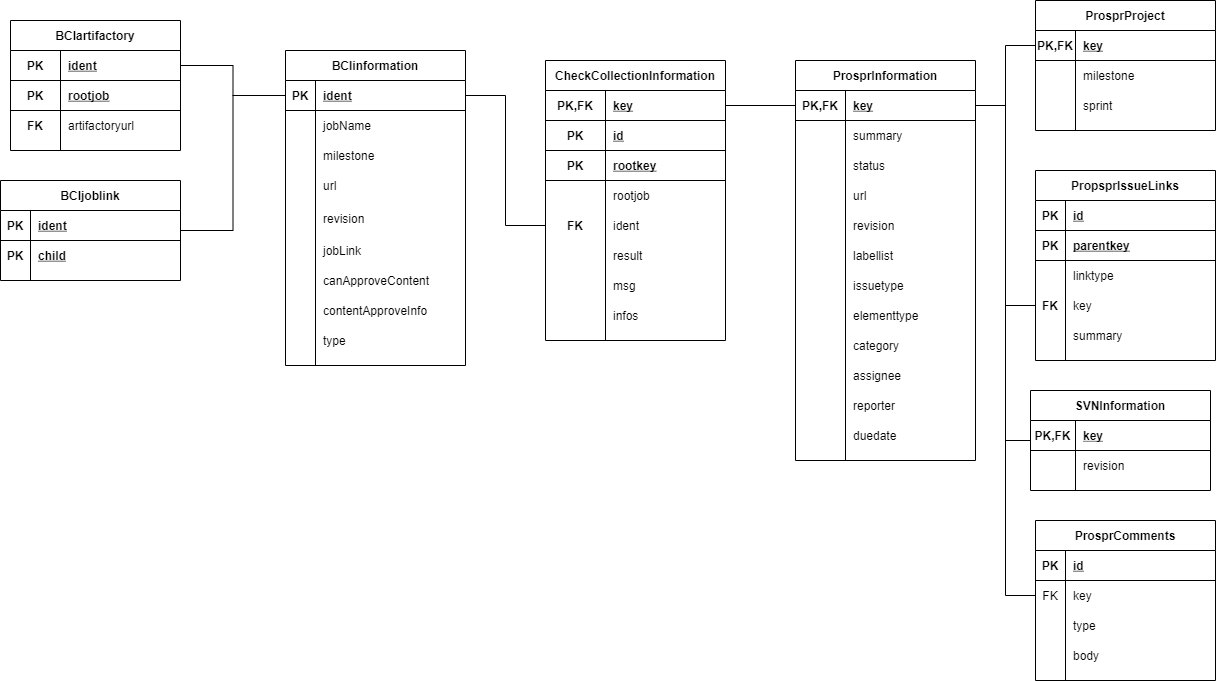
\includegraphics[width=\linewidth]{images_folder/EADBEntity.png}
    \caption{Database structure concept}
    \label{fig:dbsterconce}
\end{figure}
Given this constraints the structure in the database is simplistic. The main flaw that required a second data organization via SQL queries is mainly related to that. Data is taken as it is in code most of the time is in an unstructured format.\\
This make the process of integrating data easier, but the work that needs to be done after more complex.In Figure \ref{fig:dbsterconce} the first structure given in the database can be seen.
\begin{figure}[H]
    \centering
    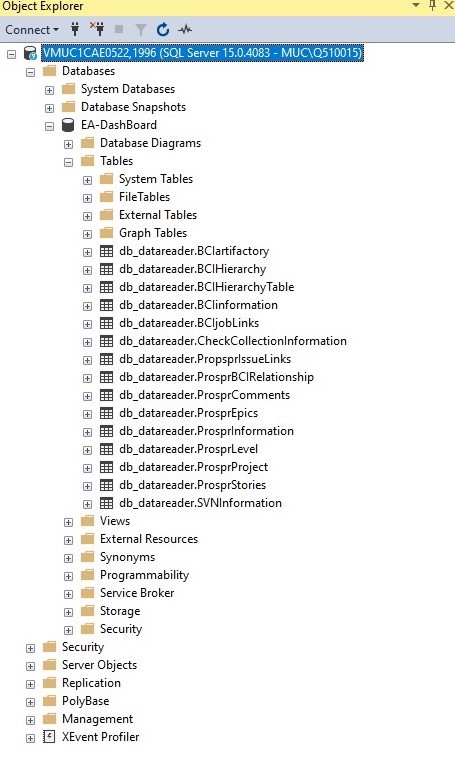
\includegraphics[width=0.5\linewidth]{images_folder/databasetable.jpg}
    \caption{Database tables}
    \label{fig:dbtables}
\end{figure} 

\section{Data Visualization}
In this section the data visualization tool is presented, as well as the concept used to create the Dashboard. 
\subsection{QlikSense}
QlikSense is a data analytic platform used to create interactive Dashboards and reports. The tools allows connection with different data sources, from excel sheets to database. The tool also include a scripting part, were SQL like language allows to query and manipulate data to create structured tables. From the structured table is then possible to create graphical visualisation of the data with interactive data search. The tool allow to develop interactive Dashboard without the need of coding the graphic logic, but just the data structure behind the visualization.\\
QlikSense is structured in three main parts, that follow the data flow from raw data to the Dashboard and reports for customers or stakeholders:
\begin{itemize}
    \item Prepare, part in which the data is loaded and the table structure is created via a SQL flavored language. 
    \item Analyze, part in which the visualization is created, different visualization schemes and menus are presents. The graphic is mainly drag and drop but allow for a Python like scripting to interface and insert formulas and conditions in the graphics.
    \item Narrate, part in which reports can be created form the Dashboard. Reporting ability is crucial to have report arriving directly to the developer.  
\end{itemize}
\subsection{Double primary key layer}
Since QlikSense allow for a SQL like table structuring, based on table connected via key during the project it has been decided to manipulate the data in the QlikSense environment.\\
This allows to keep the structure in the database simple, thus avoiding having data manipulation in the Python, one of the project requirements.\\
The data structuring is done in QlikSense via the SQL like code. The tables are loaded from the database and then modified. An example is reported in Figure \ref{fig:doublelayer}, where the software structure is imported in a parent in parent child manner. The hierarchical structure is then created via SQL queries in QlikSense.  
\begin{figure}[H]
    \centering
    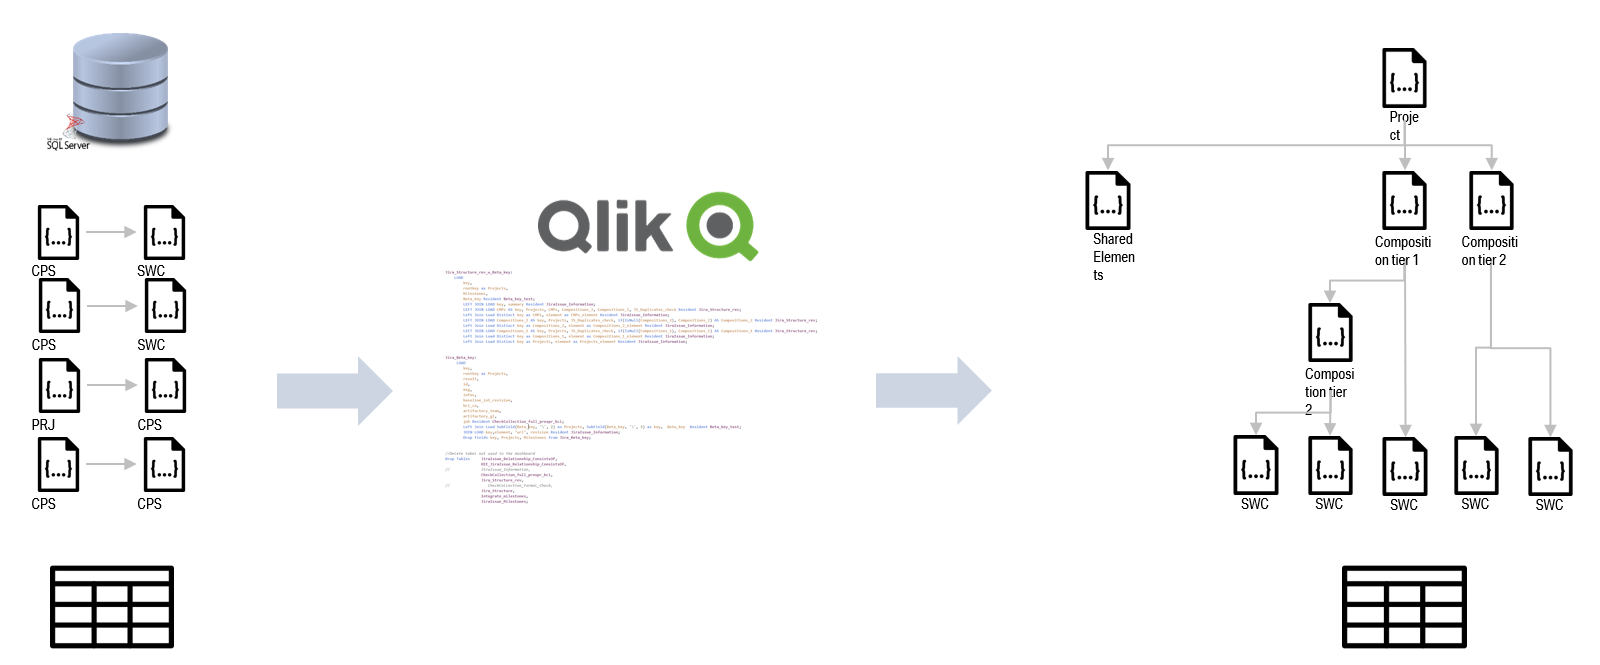
\includegraphics[width=\linewidth]{images_folder/doublalayer.png}
    \caption{Double layer primary key}
    \label{fig:doublelayer}
\end{figure} 
The concept of double layering for primary keys reports the idea that a primary key is defined both in the relational database environment. This primary key has the function of handling the update from the data generation, in terms that does not allow duplicate data to be uploaded and define a initial data structure, not related to the visualization. The table in the database are uploaded as single non linked instances in the QlikSense environment. Here a second primary key is defined, connecting the reorganized data. This primary key is the one in charge of connecting the data and allowing for surfing thought the data in a interactive manner. 
Using a double primary key layering allows, therefor for the following advantages:
\begin{itemize}
\item Have less changes in the production code for integrating of database connection and data generation.
\item During test and development phases having code defining the primary key connection in the QlikSense environment allow for a more flexibility, especially considering that in a database environment is more complex to redefine the table primary key. 
\end{itemize}
\subsection{EA Software Dashboard}
The final product of the pipeline is the Dashboard. In it the data is visualized in a graphical manner. This tool is specifically useful because it allow developer to have a direct graphic feedback on the status of software version. The data greatly vary from the RAM usage percentage of a certain Project all the way to the number of Misra rules not abode during static code analysis.\\
The variety of data is big, but almost all the data is connected to the software structure allowing for a easy search through the data.\\
There is a central menu, in which the functional area of data, or sections can be selected, in general each data section is composed by three pages, divided as follows:
\begin{itemize}
    \item Home page, where mainly general \gls{KPI} are shown and a selector for the data is present.
    \item Overview page, with graphical visualization of the data, graphs and other interactive visualization without any in depth information.
    \item In depth table, table with all the information regarding a certain data section. Most of the time a link to the production files is here preset, in case the data regards a downloadable package. 
\end{itemize}
With this organization the idea is that the developer filter the data in the first two pages, only selecting the data of interest, while in case of a more in depth information are required those can be found in the third page.  
\begin{figure}[H]
    \centering
    \includegraphics[width=\linewidth]{images_folder/Dashboard.png}
    \caption{Some of the Dashboard pages}
    \label{fig:Dashboardseite}
\end{figure}
\cleardoublepage
\end{document}